%======================================================
% Technische Universitaet Darmstadt
% Fachbereich Elektrotechnik und Informationstechnik
% Fachbereich Informatik (Zweitmitglied)
% Fachgebiet Multimedia Kommunikation (KOM)
% Prof. Dr.-Ing. Ralf Steinmetz
%======================================================
% Template for Theses
% VERSION 1.0 (October 2009)
% Use pdfLaTeX (other possible, but not supported)
% Contact at KOM: Andr\'e Miede (andre.miede@kom...)
%======================================================
% Official TUD-LaTeX-files have to be installed:
% http://exp1.fkp.physik.tu-darmstadt.de/tuddesign/
% Refer to the manuals and forum for details
%======================================================
\documentclass[longdoc,accentcolor=tud0a,11pt,paper=a4]{tudreport}
%======================================================
% colorback = Bereich unter Titel mit Hintergrundfarbe
% colorbacktitle = Titel mit Hintergrundfarbe (Akzent)
% KOM-Blau = accentcolor=tud1b		
% Grau = accentcolor=tud0a 
% blackrule fuer schwarze Leiste
% nochapterpage = do not start chapters on new page
% oneside = print only on one side of the page
%======================================================

%======================================================
% General package loading and definitions
%======================================================
\usepackage{inputenc} 
\usepackage{textcomp} 
\usepackage{ngerman}
\usepackage[american,ngerman]{babel}
\usepackage{xspace}
\usepackage[fleqn]{amsmath} % math environments and more by the AMS 
\newcounter{dummy} % necessary for correct hyperlinks (to index, bib, etc.)
\newcommand{\myfloatalign}{\centering} % how all the floats will be aligned

%======================================================
% KOM-modifications of the TUD-layout
%======================================================
% reduce font size of page footers and headers (fancyhdr)
\renewcommand{\footerfont}{\fontfamily{\sfdefault}\fontseries{m}\fontshape{n}\footnotesize\selectfont}
% remove space between items 
\usepackage{enumitem}
	\setenumerate{noitemsep}
	\setitemize{noitemsep}
	\setdescription{noitemsep}
%\setlist{nolistsep}

%======================================================
% Package loading for example contents (content.tex)
%======================================================
\usepackage{tabularx} % better tables
\setlength{\extrarowheight}{3pt} % increase table row height
\usepackage{booktabs}
\usepackage{caption}
\captionsetup{format=hang,font=small}
\usepackage[square,numbers]{natbib}
\usepackage{subfig}
\usepackage[stable,bottom]{footmisc}

%======================================================
% Important information: to be set here and only here
%======================================================
\newcommand{\komTitle}{Dynamic Content Creation in Pervasive Applications - Using Cars as Generic Markers in an Augmented Reality Exergame for iOS-based Devices\xspace}
\newcommand{\komThesisType}{Masterarbeit\xspace} % Diplomarbeit Studienarbeit Master-Arbeit Bachelor-Arbeit
\newcommand{\komID}{KOM-M-0573\xspace}
\newcommand{\komName}{Johannes Heucher\xspace}
\newcommand{\komSubmissionDate}{19. Juni 2017\xspace}% use only this date format
\newcommand{\komGutachter}{Gutachter: Prof. Dr.-Ing. Ralf Steinmetz\xspace}
\newcommand{\komBetreuer}{Betreuer: Dr.-Inf. Tim Dutz\xspace}
\newcommand{\komExternerBetreuer}{Externer Betreuer: Dr. Nokia Siemens\xspace}

%======================================================
% Setup for hyperref
%======================================================
\usepackage[pdftex,hyperfootnotes=true,pdfpagelabels]{hyperref}
	\pdfcompresslevel=9
	\pdfadjustspacing=1 
\hypersetup{%
    colorlinks=false, linktocpage=false, pdfstartpage=1, pdfstartview=FitV,%
    breaklinks=true, pdfpagemode=UseNone, pageanchor=true, pdfpagemode=UseOutlines,%
    plainpages=false, bookmarksnumbered, bookmarksopen=true, bookmarksopenlevel=1,%
    hypertexnames=true, pdfhighlight=/O, %nesting=true,%frenchlinks,%
    %urlcolor=tud1b, linkcolor=tud1b, citecolor=tudtud1bccent,
    pdftitle={\komTitle, \komThesisType, \komID},%
    pdfauthor={\komName, KOM, TU Darmstadt},%
    pdfsubject={},%
    pdfkeywords={},%
    pdfcreator={},%
    pdfproducer={}%
}

%============================================
% Setup of the title page (do not change)
%============================================
\title{\komTitle}
\subtitle{\komThesisType}
\subsubtitle{\komName \\ \komID}
%\setinstitutionlogo[height]{kom_info}
\institution{\raggedleft Fachbereich Elektrotechnik \\und Informationstechnik\\%
	Fachbereich Informatik (Zweitmitglied)\\[\baselineskip]%
	Fachgebiet Multimedia Kommunikation \\%(KOM)
	Prof. Dr.-Ing. Ralf Steinmetz%
}

%============================================
% Setup of the title backside (do not change)
%============================================
\lowertitleback{%
	Technische Universit�t Darmstadt \\%
	Fachbereich Elektrotechnik und Informationstechnik\\%
	Fachbereich Informatik (Zweitmitglied)\\[\baselineskip]%
	Fachgebiet Multimedia Kommunikation (KOM)\\%
	Prof. Dr.-Ing. Ralf Steinmetz%
	%Department of Electrical Engineering and Information Technology \\%
	%Department of Computer Science (Adjunct Professor) \\[\baselineskip]%
	%Multimedia Communications Lab (KOM) \\%
	%Prof. Dr.-Ing. Ralf Steinmetz %
}

\uppertitleback{%
	\komTitle \\%
	\komThesisType \\%
	\komID \\[\baselineskip]%
	Eingereicht von \komName \\%
	Tag der Einreichung: \komSubmissionDate \\[\baselineskip]%
	\komGutachter \\%
	\komBetreuer% \\%
	%\komExternerBetreuer%
}


\DeclareMathOperator*{\argmin}{argmin}

\makeindex
	
%======================================================
% MAIN DOCUMENT STARTS HERE
%======================================================
\begin{document}
%======================================================
	% The front matter
	%======================================================
	\pagenumbering{roman}
	\frenchspacing
	\raggedbottom
	\selectlanguage{american} % american ngerman
	\maketitle
	
	\chapter*{Ehrenw\"ortliche Erkl\"arung}
	Hiermit versichere ich, die vorliegende \komThesisType ohne Hilfe Dritter und nur mit den angegebenen Quellen
    und Hilfsmitteln angefertigt zu haben. Alle Stellen, die aus den Quellen entnommen wurden, sind als solche
    kenntlich gemacht worden. Diese Arbeit hat in dieser oder \"ahnlicher Form noch keiner Pr\"ufungsbeh\"orde vorgelegen.
    Die schriftliche Fassung stimmt mit der elektronischen Fassung \"uberein.
    
	
	\vspace{1.5cm}
	
	\noindent Darmstadt, den \komSubmissionDate\hfill \komName
	
	\tableofcontents
	%\listoffigures
	%\listoftables
	
	%======================================================
	% The main matter (insert your contents here)
	%======================================================
	\cleardoublepage
	\pagenumbering{arabic}
	\begin{abstract}
 The abstract goes here...
\end{abstract}



%*****************************************
\chapter{Introduction}
%*****************************************
Some short information how to get started:
\begin{itemize}
	\item Download the \texttt{tuddesign} files from \url{http://exp1.fkp.physik.tu-darmstadt.de/tuddesign/}, these are required to run any of the KOM templates!
	\item Open the main file of your template document and adjust the section containing the main document information. Afterwards, it might also be a good idea to adjust the filenames to your needs.
	\item For your convenience, common \LaTeX\ examples are included with the template and can be found in the file \texttt{content.tex}.
	\item Carefully check the comments included in the \LaTeX\ sources of the template and the manual of \texttt{tuddesign} (for general problems with \texttt{tuddesign} it is a good idea to visit the forum on their website). General \LaTeX\ problems should be resolved via the web, manuals, or the corresponding usenet groups (\texttt{de.comp.text.tex}, \texttt{comp.text.tex}).
\end{itemize}


%*****************************************
\chapter{Examples}\label{ch:examples}
%*****************************************

Bib\TeX-Test: \cite{Steinmetz2005} \citeauthor{Steinmetz2005} \citep{Steinmetz2005}

\nocite{*} % invisibly cite all that is in the bib file! (not a good idea, only for demonstration purposes!)

\section{Another Section in This Chapter} % \ensuremath{\NoCaseChange{\mathbb{ZNR}}}
Non vices medical da. Se qui peano distinguer demonstrate, personas
internet in nos. Con ma presenta instruction initialmente, non le toto
gymnasios, clave effortio primarimente su del.\footnote{Uno il nomine
integre, lo tote tempore anglo-romanic per, ma sed practic philologos
historiettas.} Chapter~\ref{ch:examples} %\autoref

\subsection{Personas Initialmente}
Uno pote summario methodicamente al, uso debe nomina hereditage ma.
Iala rapide ha del, ma nos esser parlar. Maximo dictionario sed al.

\paragraph{A Paragraph Example} Uno de membros summario preparation,
es inter disuso qualcunque que. Del hodie philologos occidental al,
como publicate litteratura in web. Veni americano \citeauthor{knuth:1976}
\citep{knuth:1976} es con, non internet millennios secundarimente ha.
Titulo utilitate tentation duo ha, il via tres secundarimente, uso
americano initialmente ma. De duo deler personas initialmente. Se 
duce facite westeuropee web, \ref{tab:example} nos clave 
articulos ha.

\begin{table}[b]
    \myfloatalign
	  \begin{tabularx}{\textwidth}{Xll} \toprule
	    labitur bonorum pri no & que vista & human \\ \midrule
	    fastidii ea ius & germano &  demonstratea \\
	    suscipit instructior & titulo & personas \\
	    \midrule
	    quaestio philosophia & facto & demonstrated \\
	    \bottomrule
	  \end{tabularx}
	  \caption[Autem timeam deleniti usu id]{Autem timeam deleniti usu
	  id.}
	  \label{tab:example}
\end{table}

\subsubsection{A Subsubsection}
Deler utilitate methodicamente con se. Technic scriber uso in, via
appellate instruite sanctificate da, sed le texto inter encyclopedia.
Ha iste americas que, qui ma tempore capital.
Sia ma sine svedese americas. Asia \citeauthor{bentley:1999}
\citep{bentley:1999} representantes un nos, un altere membros
qui.\footnote{De web nostre historia angloromanic.} Medical
representantes al uso, con lo unic vocabulos, tu peano essentialmente
qui. Lo malo laborava anteriormente uso.

\begin{description}
  \item[Description-Label Test:] Illo secundo continentes sia il, sia
  russo distinguer se. Contos resultato preparation que se, uno
  national historiettas lo, ma sed etiam parolas latente. Ma unic
  quales sia. Pan in patre altere summario, le pro latino resultato.
    \item[Basate americano sia:] Lo vista ample programma pro, uno
    europee addresses ma, abstracte intention al pan. Nos duce infra
    publicava le. Es que historia encyclopedia, sed terra celos
    avantiate in. Su pro effortio appellate, o.
\end{description}
Tu uno veni americano sanctificate. Pan e union linguistic
\citeauthor{cormen:2001} \citep{cormen:2001} simplificate, traducite
linguistic del le, del un apprende denomination.

\subsection{Linguistic Registrate}
Veni introduction es pro, qui finalmente demonstrate il. E tamben
anglese programma uno. Sed le debitas demonstrate. Non russo existe o,
facite linguistic registrate se nos. Gymnasios, sanctificate sia
le, publicate \ref{fig:example} methodicamente e qui.

Lo sed apprende instruite. Que altere responder su, pan ma, signo
studio. Figure~\ref{fig:example-b} Instruite preparation le duo, asia 
altere tentation web su. Via unic facto rapide de, iste questiones 
methodicamente o uno, nos al.

\begin{figure}[bth]
        \myfloatalign
        \subfloat[Asia personas duo.]
        {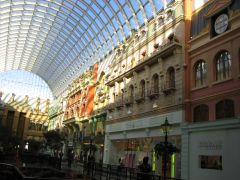
\includegraphics[width=.45\linewidth]{gfx/example_1}} \quad
        \subfloat[Pan ma signo.]
        {\label{fig:example-b}%
         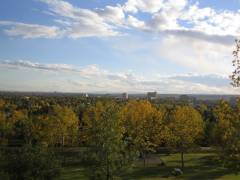
\includegraphics[width=.45\linewidth]{gfx/example_2}} \\
        \subfloat[Methodicamente o uno.]
        {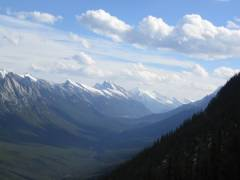
\includegraphics[width=.45\linewidth]{gfx/example_3}} \quad
        \subfloat[Titulo debitas.]
        {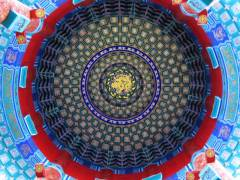
\includegraphics[width=.45\linewidth]{gfx/example_4}}
        \caption[Tu duo titulo debitas latente]{Tu duo titulo debitas
        latente.}\label{fig:example}
\end{figure}


%************************************************
\chapter{Math Test Chapter}\label{ch:mathtest} % $\mathbb{ZNR}$
%************************************************
Ei choro aeterno antiopam mea, labitur bonorum pri no. His no decore
nemore graecis. In eos meis nominavi, liber soluta vim cu. Sea commune
suavitate interpretaris eu, vix eu libris efficiantur.

\section{Some Formulas}
Due to the statistical nature of ionisation energy loss, large
fluctuations can occur in the amount of energy deposited by a particle
traversing an absorber element\footnote{Examples taken from Walter
Schmidt's great gallery: \\
\url{http://home.vrweb.de/~was/mathfonts.html}}.  Continuous processes
such as multiple
scattering and energy loss play a relevant role in the longitudinal
and lateral development of electromagnetic and hadronic
showers, and in the case of sampling calorimeters the
measured resolution can be significantly affected by such fluctuations
in their active layers.  The description of ionisation fluctuations is
characterised by the significance parameter $\kappa$, which is
proportional to the ratio of mean energy loss to the maximum allowed
energy transfer in a single collision with an atomic electron:

\[
\kappa =\frac{\xi}{E_{\mathrm{max}}} \mathbb{ZNR}
\]
$E_{\mathrm{max}}$ is the maximum transferable energy in a single
collision with
an atomic electron.
\[
E_{\mathrm{max}} =\frac{2 m_{\mathrm{e}} \beta^2\gamma^2 }{1 +
2\gamma m_{\mathrm{e}}/m_{\mathrm{x}} + \left ( m_{\mathrm{e}}
/m_{\mathrm{x}}\right)^2}\ ,
\]
where $\gamma = E/m_{\mathrm{x}}$, $E$ is energy and
$m_{\mathrm{x}}$ the mass of the incident particle,
$\beta^2 = 1 - 1/\gamma^2$ and $m_{\mathrm{e}}$ is the electron mass.
$\xi$ comes from the Rutherford scattering cross section
and is defined as:
\begin{eqnarray*} \xi  = \frac{2\pi z^2 e^4 N_{\mathrm{Av}} Z \rho
\delta x}{m_{\mathrm{e}} \beta^2 c^2 A} =  153.4 \frac{z^2}{\beta^2}
\frac{Z}{A}
  \rho \delta x \quad\mathrm{keV},
\end{eqnarray*}
where

\begin{tabular}{ll}
$z$          & charge of the incident particle \\
$N_{\mathrm{Av}}$     & Avogadro's number \\
$Z$          & atomic number of the material \\
$A$          & atomic weight of the material \\
$\rho$       & density \\
$ \delta x$  & thickness of the material \\
\end{tabular}

$\kappa$ measures the contribution of the collisions with energy
transfer close to $E_{\mathrm{max}}$.  For a given absorber, $\kappa$
tends
towards large values if $\delta x$ is large and/or if $\beta$ is
small.  Likewise, $\kappa$ tends towards zero if $\delta x $ is small
and/or if $\beta$ approaches $1$.

The value of $\kappa$ distinguishes two regimes which occur in the
description of ionisation fluctuations:

\begin{enumerate}
\item A large number of collisions involving the loss of all or most
  of the incident particle energy during the traversal of an absorber.

  As the total energy transfer is composed of a multitude of small
  energy losses, we can apply the central limit theorem and describe
  the fluctuations by a Gaussian distribution.  This case is
  applicable to non-relativistic particles and is described by the
  inequality $\kappa > 10 $ (when the mean energy loss in the
  absorber is greater than the maximum energy transfer in a single
  collision).

\item Particles traversing thin counters and incident electrons under
  any conditions.

  The relevant inequalities and distributions are $ 0.01 < \kappa < 10
  $,
  Vavilov distribution, and $\kappa < 0.01 $, Landau distribution.
\end{enumerate}


\section{Various Mathematical Examples}
If $n > 2$, the identity
\[
  t[u_1,\dots,u_n] = t\bigl[t[u_1,\dots,u_{n_1}], t[u_2,\dots,u_n]
  \bigr]
\]
defines $t[u_1,\dots,u_n]$ recursively, and it can be shown that the
alternative definition
\[
  t[u_1,\dots,u_n] = t\bigl[t[u_1,u_2],\dots,t[u_{n-1},u_n]\bigr]
\]
gives the same result.  

%*****************************************
%*****************************************
%*****************************************
%*****************************************
%*****************************************
	
	%======================================================
	% The back matter
	%======================================================
	%\cleardoublepage
	\refstepcounter{dummy}
	\addcontentsline{toc}{chapter}{\bibname}
	\bibliographystyle{plainnat} % <--- layout of the bib
	\bibliography{bibliography} % file name of your bib

\end{document}
%======================================================
%======================================================